\section{TP 0 : Introduction à la programmation avec Scratch}


\begin{UPSTIinfor}{Objectif du TP}
Pour cette semaine 0, nous allons (re)découvrir les bases de la programmation à travers le langage Scratch. 

L'utilisation de Scratch nous permettra de nous familiariser avec les concepts fondamentaux de la programmation sans avoir à se soucier de la syntaxe complexe des langages de programmation traditionnels.

A la fin de cette séance, vous connaitrez les principaux concepts de la programmation :
\begin{itemize}
\item Variables
\item Boucles
\item Conditions
\end{itemize}
Durant toute cette séance, s'il y a le moindre détail qui n'est pas clair pour vous, n'hésitez pas à poser une question à l'enseignant ou à un camarade.
\end{UPSTIinfor}

\begin{UPSTIidee}{Je sais déjà programmer, est-ce que je peux passer ce TP ?}

Si vous avez déjà une expérience de programmation, les premiers exercices vous paraitront très simples. Faites alors le dernier exercice de chaque section et faites le valider par l'enseignant. 
Vous pourrez alors choisir un problème de niveau avancé.
\end{UPSTIidee}

\begin{UPSTIwarning}{Anglais ou français ?}
Sur cette page, les images des blocs sont en anglais. Vous pouvez utiliser Scratch dans la langue de votre choix.
\end{UPSTIwarning}


\subsection{Présentation de l'interface}

\begin{figure}[h]
\centering
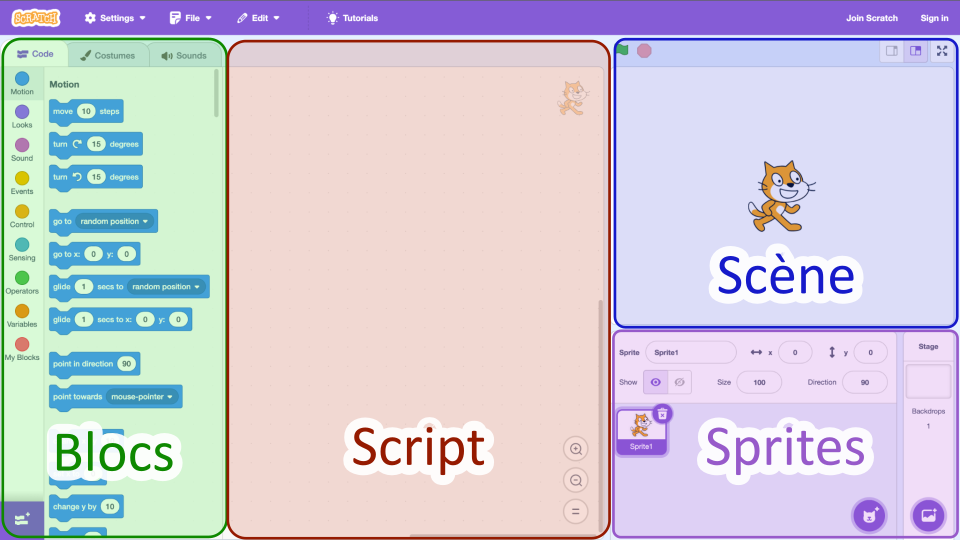
\includegraphics[width=0.8\textwidth]{scratch_description.png}
\caption{scratch interface décrite}
\end{figure}

L'interface de Scratch est divisée en plusieurs sections :
\begin{itemize}
\item \textbf{Palette de blocs} : où vous trouverez les différents blocs de code que vous pouvez utiliser
\item \textbf{Mouvement} : pour déplacer les sprites
\item \textbf{Apparence} : pour modifier l'apparence des sprites
\item \textbf{Événements} : pour déclencher des actions
\item \textbf{Contrôle} : pour gérer le flux du programme
\item \textbf{Sons} : pour ajouter des effets sonores
\item \textbf{Zone de script} : où vous assemblez les blocs pour créer votre programme
\item \textbf{Zone de scène} : où vous pouvez voir votre projet en action
\item \textbf{Liste des sprites} : où vous pouvez ajouter ou sélectionner les sprites de votre projet
\end{itemize}
